\documentclass[10pt,a4paper]{article}
\usepackage[a4paper,margin=1.55cm,top=1.4cm,bottom=1.5cm]{geometry}
\usepackage[T1]{fontenc}
\usepackage{lmodern}
\usepackage{microtype}
\usepackage{graphicx}
\usepackage{booktabs}
\usepackage{tabularx}
\usepackage{xcolor}
\usepackage{enumitem}
\usepackage{caption}
\usepackage{titlesec}
\usepackage[hidelinks]{hyperref}

\definecolor{plum}{HTML}{7D4570}
\definecolor{ink}{HTML}{1D161B}
\definecolor{muted}{HTML}{6B6169}
\hypersetup{colorlinks=true,urlcolor=plum,linkcolor=plum}
\captionsetup{font=small,labelfont={bf,color=plum},skip=3pt}
\titleformat{\section}{\large\bfseries\color{plum}}{\thesection}{0.6em}{}
\titlespacing*{\section}{0pt}{7pt}{3pt}
\setlist{nosep,leftmargin=1.2em}
\setlength{\parskip}{3pt}
\setlength{\parindent}{0pt}
\renewcommand{\arraystretch}{1.08}

% generated by dpcn/report_numbers.py -- do not edit
\newcommand{\FacListed}{410}
\newcommand{\FacMatched}{397}
\newcommand{\FacMatchPct}{96.8\%}
\newcommand{\Papers}{11,639}
\newcommand{\TopTenPlanck}{Seven}
\newcommand{\Rows}{12,277}
\newcommand{\AffRowsPct}{67\%}
\newcommand{\DoiPct}{98.1\%}
\newcommand{\QuartPct}{93.3\%}
\newcommand{\CitEdges}{84,879}
\newcommand{\CoPairs}{49,154}
\newcommand{\PartnerRows}{542}
\newcommand{\HyperCap}{50}
\newcommand{\PapB}{3,186}
\newcommand{\CitB}{52,576}
\newcommand{\CitNoHypB}{52,197}
\newcommand{\HypB}{5}
\newcommand{\QOneB}{73.5\%}
\newcommand{\CAGRB}{12.2\%}
\newcommand{\FWCIB}{0.88}
\newcommand{\TopTenB}{16.5\%}
\newcommand{\IntlB}{26\%}
\newcommand{\OAB}{44\%}
\newcommand{\GiniB}{0.65}
\newcommand{\GrowthB}{14.7\%}
\newcommand{\GrowthPB}{0.000}
\newcommand{\CovidB}{-3.5\%}
\newcommand{\CovidPB}{0.84}
\newcommand{\MKB}{increasing}
\newcommand{\ConfB}{208}
\newcommand{\HMedB}{12}
\newcommand{\NFacB}{160}
\newcommand{\InB}{12,444}
\newcommand{\OutB}{21,207}
\newcommand{\RatioB}{0.59}
\newcommand{\PartnersB}{367}
\newcommand{\TopCiterB}{Academy of Scientific and Innovative Research}
\newcommand{\TopPartnerB}{Indian Institute of Technology Kanpur}
\newcommand{\TopJB}{Physical Review B}
\newcommand{\TopJNB}{122}
\newcommand{\PapM}{2,443}
\newcommand{\CitM}{43,294}
\newcommand{\CitNoHypM}{39,210}
\newcommand{\HypM}{120}
\newcommand{\QOneM}{74.2\%}
\newcommand{\CAGRM}{8.1\%}
\newcommand{\FWCIM}{0.81}
\newcommand{\TopTenM}{14.7\%}
\newcommand{\IntlM}{27\%}
\newcommand{\OAM}{48\%}
\newcommand{\GiniM}{0.66}
\newcommand{\GrowthM}{8.0\%}
\newcommand{\GrowthPM}{0.003}
\newcommand{\CovidM}{9.4\%}
\newcommand{\CovidPM}{0.63}
\newcommand{\MKM}{increasing}
\newcommand{\ConfM}{49}
\newcommand{\HMedM}{15}
\newcommand{\NFacM}{118}
\newcommand{\InM}{11,485}
\newcommand{\OutM}{16,340}
\newcommand{\RatioM}{0.70}
\newcommand{\PartnersM}{282}
\newcommand{\TopCiterM}{Academy of Scientific and Innovative Research}
\newcommand{\TopPartnerM}{Tata Institute of Fundamental Research}
\newcommand{\TopJM}{Physical Review D}
\newcommand{\TopJNM}{96}
\newcommand{\PapT}{2,014}
\newcommand{\CitT}{53,136}
\newcommand{\CitNoHypT}{27,441}
\newcommand{\HypT}{36}
\newcommand{\QOneT}{73.7\%}
\newcommand{\CAGRT}{16.7\%}
\newcommand{\FWCIT}{0.73}
\newcommand{\TopTenT}{14.8\%}
\newcommand{\IntlT}{30\%}
\newcommand{\OAT}{41\%}
\newcommand{\GiniT}{0.82}
\newcommand{\GrowthT}{17.7\%}
\newcommand{\GrowthPT}{0.000}
\newcommand{\CovidT}{11.6\%}
\newcommand{\CovidPT}{0.56}
\newcommand{\MKT}{increasing}
\newcommand{\ConfT}{60}
\newcommand{\HMedT}{12}
\newcommand{\NFacT}{119}
\newcommand{\InT}{8,745}
\newcommand{\OutT}{9,000}
\newcommand{\RatioT}{0.97}
\newcommand{\PartnersT}{245}
\newcommand{\TopCiterT}{Homi Bhabha National Institute}
\newcommand{\TopPartnerT}{Indian Institute of Science Bangalore}
\newcommand{\TopJT}{Angewandte Chemie}
\newcommand{\TopJNT}{58}
\newcommand{\PapAll}{7,597}
\newcommand{\CitAll}{148,485}
\newcommand{\CitNoHypAll}{118,327}
\newcommand{\HypAll}{161}
\newcommand{\QOneAll}{73.7\%}
\newcommand{\CAGRAll}{12.0\%}
\newcommand{\FWCIAll}{0.81}
\newcommand{\TopTenAll}{15.5\%}
\newcommand{\IntlAll}{27\%}
\newcommand{\OAAll}{45\%}
\newcommand{\GiniAll}{0.72}
\newcommand{\GrowthAll}{13.1\%}
\newcommand{\GrowthPAll}{0.000}
\newcommand{\CovidAll}{3.7\%}
\newcommand{\CovidPAll}{0.84}
\newcommand{\MKAll}{increasing}
\newcommand{\ConfAll}{317}
\newcommand{\KWH}{3.44}
\newcommand{\KWP}{0.179}
\newcommand{\ChiSq}{2.7}
\newcommand{\ChiP}{0.85}
\newcommand{\CramerV}{0.014}
\newcommand{\FwciH}{15.0}
\newcommand{\FwciP}{0.00055}
\newcommand{\TeamRho}{0.20}
\newcommand{\CNodes}{7,597}
\newcommand{\CEdges}{17,386}
\newcommand{\CGiant}{51\%}
\newcommand{\CSelf}{96\%}
\newcommand{\CLag}{2}
\newcommand{\CAlpha}{2.97}
\newcommand{\CXmin}{6}
\newcommand{\CRLN}{-3.92}
\newcommand{\CPLN}{0.00}
\newcommand{\CREXP}{-0.3}
\newcommand{\CPEXP}{0.76}
\newcommand{\CInIndia}{26,854}
\newcommand{\COutIndia}{40,639}
\newcommand{\PRTopTitle}{Superconducting properties of the noncentrosymmetric superconductor Re6Hf}
\newcommand{\PRTopYear}{2016}
\newcommand{\PRTopCoreTitle}{Superconducting properties of the noncentrosymmetric superconductor Re6Hf}
\newcommand{\ANodes}{397}
\newcommand{\AConn}{204}
\newcommand{\AEdges}{304}
\newcommand{\AIso}{193}
\newcommand{\AMeanDeg}{3.0}
\newcommand{\AGiant}{79\%}
\newcommand{\AClust}{0.17}
\newcommand{\ALeiden}{27}
\newcommand{\AQ}{0.71}
\newcommand{\ALouvQ}{0.79}
\newcommand{\ANMI}{0.63}
\newcommand{\AARI}{0.32}
\newcommand{\AAssDept}{0.48}
\newcommand{\AAssInst}{0.85}
\newcommand{\ADegAss}{0.21}
\newcommand{\ACross}{29}
\newcommand{\AEdgesHyp}{304}
\newcommand{\ASigma}{5.8}
\newcommand{\AC}{0.19}
\newcommand{\ACnull}{0.03}
\newcommand{\AL}{4.99}
\newcommand{\ALnull}{4.11}
\newcommand{\ACratio}{7}
\newcommand{\ASigmaLo}{3.3}
\newcommand{\ASigmaHi}{18.6}
\newcommand{\AGiantStart}{14\%}
\newcommand{\AGiantEnd}{79\%}
\newcommand{\AModStart}{0.91}
\newcommand{\AModEnd}{0.72}
\newcommand{\AYearStart}{2016}
\newcommand{\AYearEnd}{2026}
\newcommand{\ABtwA}{Deepak Chopra (Chemistry, Bhopal)}
\newcommand{\ABtwB}{Sukhendu Mandal (Chemistry, TVM)}
\newcommand{\ABtwC}{Aasheesh Srivastava (Chemistry, Bhopal)}
\newcommand{\ADegA}{Deepak Chopra (13)}
\newcommand{\ADegB}{Santanu Kumar Pal (13)}
\newcommand{\ADegC}{Sukhendu Mandal (13)}
\newcommand{\LPSplit}{2022}
\newcommand{\LPPos}{44}
\newcommand{\LPAA}{0.64}
\newcommand{\LPJac}{0.64}
\newcommand{\LPPA}{0.71}
\newcommand{\LPDept}{0.70}
\newcommand{\DashURL}{https://incognius.github.io/DPCN-A2-EigenMinds/}
\newcommand{\RepoURL}{https://github.com/Incognius/DPCN-A2-EigenMinds}
\newcommand{\Partners}{542}
\newcommand{\Linked}{2,033}
\newcommand{\SimLo}{0.52}
\newcommand{\SimHi}{0.61}


\begin{document}

\noindent\begin{minipage}[t]{0.86\linewidth}
{\color{plum}\Large\bfseries Research mapping of IISER Bhopal, Mohali and Thiruvananthapuram, 2016--2026}\\[2pt]
{\color{muted}DPCN course project \textbullet{} Group 20, team \textbf{EigenMinds}: Ponnambalam V, Manit Roy, Shashwat Mukadam \textbullet{} First-round report \textbullet{} Instructor: Prof.\ Chittaranjan Hens}\\[2pt]
{\small Interactive dashboard: \url{\DashURL}\\ Code, data and network files: \url{\RepoURL}}
\end{minipage}\hfill
\begin{minipage}[t]{0.12\linewidth}\vspace{0pt}\raggedleft

\includegraphics[width=\linewidth]{figures/qr_dashboard.png}\\[-1pt]{\tiny\color{muted}dashboard}
\end{minipage}

\vspace{4pt}
\noindent\colorbox{plum!7}{\begin{minipage}{\dimexpr\linewidth-2\fboxsep}
\small\textbf{Key findings.}
\begin{itemize}
\item \textbf{Same quality, different growth.} The three IISERs publish an almost identical share of Q1 papers (\QOneB, \QOneM, \QOneT; $\chi^2$ $p=\ChiP$, Cram\'er's $V=\CramerV$), but output grows at very different rates: \CAGRT{} a year at TVM, \CAGRB{} at Bhopal and \CAGRM{} at Mohali (2016$\to$2025).
\item \textbf{A few giant papers carry the citations.} \HypAll{} papers with more than \HyperCap{} authors (Planck, pulsar timing, collider experiments) hold a fifth of all citations; TVM loses almost half its citation count without them (\CitT{} $\to$ \CitNoHypT). Field-weighted impact (FWCI) is the fair comparison, and there Bhopal leads (median \FWCIB{} vs \FWCIM{} and \FWCIT; Kruskal--Wallis $p=\FwciP$).
\item \textbf{Three islands.} \CSelf{} of citations between the three institutes' papers stay inside one institute, and only \ACross{} of \AEdges{} faculty co-authorship ties cross between them. Collaboration communities follow the institute (assortativity \AAssInst) more than the department (\AAssDept).
\item \textbf{Net importers of Indian knowledge.} Each IISER cites other Indian institutes more than they cite it back (in/out ratio \RatioB, \RatioM, \RatioT), with TVM nearly in balance.
\end{itemize}
\end{minipage}}

\section{Data and method}
\textbf{Faculty.} We scraped the current regular faculty (Assistant, Associate and full Professors) from each institute's own website: Bhopal's ten department sites, Mohali's \emph{People} page and TVM's seven school pages. That gives \FacListed{} faculty (Bhopal \NFacB, Mohali \NFacM, TVM \NFacT{} matched). Visiting, adjunct, emeritus and fellowship posts are excluded so the institutes are counted alike. Each name was matched to an OpenAlex author profile by downloading every author OpenAlex has ever affiliated with the institute and fuzzy-matching locally, requiring both surname and given name to agree and preferring the profile whose field fits the department; \FacMatched{} (\FacMatchPct) matched.

\textbf{Papers.} We fetched all 2016--2026 journal and conference papers of the matched authors from OpenAlex: \Papers{} unique papers, giving \Rows{} faculty--paper rows in \texttt{group20\_data.csv}. Because OpenAlex lists truncate authors at 100, every larger paper was re-fetched in full. A row is \emph{affiliated} when that faculty member's authorship lists the IISER (\AffRowsPct{} of rows); institute statistics count each affiliated paper once. Journal quartiles come from SCImago, matched on ISSN and year (\QuartPct{} of journal papers covered), and conference ranks from CORE 2023. For the Indian-connection columns we fetched the institutions of all 385k referenced works and every Indian-authored work citing a corpus paper.

\textbf{Limits.} Only current faculty are listed, so papers by people who left before 2026 are missing and institute totals undercount total institutional output. Citation counts are as of October 2026.

\section{Output, quality and people}
\begin{figure}[!htb]
\centering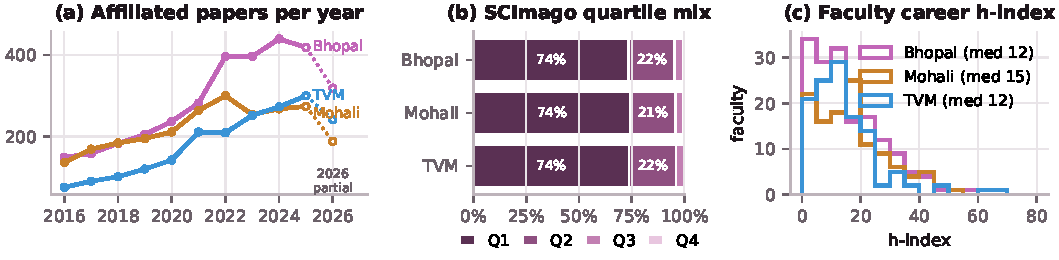
\includegraphics[width=\linewidth]{figures/fig_output.pdf}
\caption{(a) Unique affiliated papers per year; 2026 is partial. (b) SCImago quartile mix of journal papers. (c) Career h-index of current faculty (OpenAlex), with medians.}
\label{fig:output}
\end{figure}

\begin{table}[!htb]
\centering\small
\caption{Institute-level statistics (unique affiliated papers, 2016--2026).}
\label{tab:inst}
\begin{tabular}{lrrrr}
\toprule
 & Bhopal & Mohali & TVM & All three \\
\midrule
Papers & \PapB & \PapM & \PapT & \PapAll \\
Citations (excl.\ $>$\HyperCap{} authors) & \CitB{} (\CitNoHypB) & \CitM{} (\CitNoHypM) & \CitT{} (\CitNoHypT) & \CitAll{} (\CitNoHypAll) \\
Q1 share & \QOneB & \QOneM & \QOneT & \QOneAll \\
Median FWCI / top-10\% cited & \FWCIB{} / \TopTenB & \FWCIM{} / \TopTenM & \FWCIT{} / \TopTenT & \FWCIAll{} / \TopTenAll \\
NB-GLM growth per year ($p$) & \GrowthB{} (\GrowthPB) & \GrowthM{} (\GrowthPM) & \GrowthT{} (\GrowthPT) & \GrowthAll{} (\GrowthPAll) \\
COVID-years effect ($p$) & \CovidB{} (\CovidPB) & \CovidM{} (\CovidPM) & \CovidT{} (\CovidPT) & \CovidAll{} (\CovidPAll) \\
International co-authorship / OA & \IntlB{} / \OAB & \IntlM{} / \OAM & \IntlT{} / \OAT & \IntlAll{} / \OAAll \\
Citation Gini & \GiniB & \GiniM & \GiniT & \GiniAll \\
Median faculty h-index & \HMedB & \HMedM & \HMedT & -- \\
\bottomrule
\end{tabular}
\end{table}

Output rose at all three institutes (Mann--Kendall trend \MKB, \MKM, \MKT). A negative-binomial regression of yearly counts on year with a 2020--21 indicator finds significant growth everywhere but \emph{no} COVID effect at any institute (all $p>0.5$). Bhopal's jump after 2021 is broad-based: Chemistry, Physics, EECS and Earth Sciences all grew by half or more between 2019--21 and 2022--24. The quartile mix is statistically indistinguishable across institutes (Table~\ref{tab:inst}, Fig.~\ref{fig:output}b), and so is faculty h-index (Kruskal--Wallis $H=\KWH$, $p=\KWP$). The institutes differ in \emph{concentration} instead: TVM's citation Gini of \GiniT{} reflects \HypT{} large-collaboration papers, mostly Planck. Larger teams are cited more (Spearman $\rho=\TeamRho$ between author count and citations), which is one reason raw counts mislead.

\section{Journals, research areas and most-cited papers}
\begin{minipage}[t]{0.56\linewidth}
\vspace{0pt}\small
\captionof{table}{Top 5 journals per institute (papers, SCImago quartile).}
\label{tab:journals}
\begin{tabularx}{\linewidth}{@{}l X r c@{}}
\toprule
 & Journal & $n$ & Q \\
\midrule
Bhopal & Physical Review B & 122 & Q1 \\
 & Chemical Communications & 84 & Q1 \\
 & Organic Letters & 61 & Q1 \\
 & Chemistry - A European Journal & 61 & Q1 \\
 & Chemistry - An Asian Journal & 42 & Q2 \\
\addlinespace[2pt]
Mohali & Physical Review D & 96 & Q1 \\
 & Physical Review B & 41 & Q1 \\
 & Chemical Communications & 40 & Q1 \\
 & Scientific Reports & 39 & Q1 \\
 & Chemistry - A European Journal & 38 & Q1 \\
\addlinespace[2pt]
TVM & Angewandte Chemie International Edition & 56 & Q1 \\
 & Physical Review B & 53 & Q1 \\
 & Chemical Communications & 42 & Q1 \\
 & Chemistry - A European Journal & 37 & Q1 \\
 & The Journal of Physical Chemistry C & 35 & Q1 \\
\bottomrule

\end{tabularx}
\end{minipage}\hfill
\begin{minipage}[t]{0.41\linewidth}
\vspace{0pt}
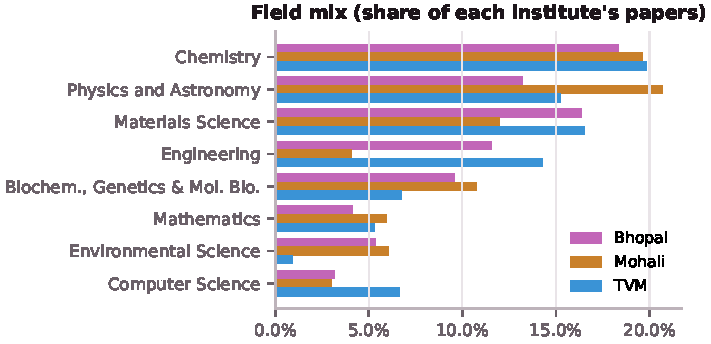
\includegraphics[width=\linewidth]{figures/fig_fields.pdf}
\captionof{figure}{Research-area breakdown: share of each institute's papers in the eight largest OpenAlex fields.}
\label{fig:fields}
\end{minipage}

\vspace{4pt}
Chemistry is the largest field at Bhopal and TVM (about a fifth of papers) and level with physics at Mohali, the most physics-heavy of the three. Bhopal and TVM put more into materials science and engineering. Earth and environmental science is about a tenth of Bhopal's and Mohali's output but under 2\% of TVM's (Fig.~\ref{fig:fields}). The physics venues (\emph{Physical Review B} and \emph{D}) and the chemistry venues (\emph{Angewandte}, \emph{Chem.\ Commun.}, \emph{Chem.\ Eur.\ J.}) dominate the publication lists (Table~\ref{tab:journals}).

\begin{table}[!htb]
\centering\footnotesize
\caption{The ten most-cited papers (all three IISERs, citations to October 2026). \TopTenPlanck{} are parts of the \emph{Planck 2018} release; excluding papers with more than \HyperCap{} authors, the top paper is a 2020 \emph{Advanced Functional Materials} paper on post-synthetic modification of metal--organic frameworks (dashboard: Journals \& Impact, ``$\le$ 50 authors'').}
\label{tab:cited}
\begin{tabularx}{\linewidth}{@{}r X l r r l@{}}
\toprule
\# & Title & Venue & Year & Cites & DOI \\
\midrule
1 & Planck 2018 results & Astronomy and Astrophysics & 2020 & 14,257 & \texttt{\scriptsize 10.1051/0004-6361/201833910} \\
2 & Planck 2018 results & Astronomy and Astrophysics & 2019 & 2,426 & \texttt{\scriptsize 10.1051/0004-6361/201833887} \\
3 & Planck 2018 results & Astronomy and Astrophysics & 2019 & 1,636 & \texttt{\scriptsize 10.1051/0004-6361/201833880} \\
4 & Planck 2018 results & Astronomy and Astrophysics & 2020 & 1,192 & \texttt{\scriptsize 10.1051/0004-6361/201936386} \\
5 & Planck 2018 results & Astronomy and Astrophysics & 2019 & 781 & \texttt{\scriptsize 10.1051/0004-6361/201833886} \\
6 & Planck 2018 results & Astronomy and Astrophysics & 2020 & 696 & \texttt{\scriptsize 10.1051/0004-6361/201935891} \\
7 & Post‐Synthetic Modification of Metal–Organic Frameworks Towar… & Advanced Functional Mater… & 2020 & 645 & \texttt{\scriptsize 10.1002/adfm.202006291} \\
8 & Models and materials for generalized Kitaev magnetism & Journal of Physics Conden… & 2017 & 613 & \texttt{\scriptsize 10.1088/1361-648x/aa8cf5} \\
9 & Tropospheric Ozone Assessment Report: Present-day tropospheri… & Elementa Science of the A… & 2018 & 592 & \texttt{\scriptsize 10.1525/elementa.302} \\
10 & Planck 2018 results & Astronomy and Astrophysics & 2019 & 484 & \texttt{\scriptsize 10.1051/0004-6361/201935201} \\
\bottomrule

\end{tabularx}
\end{table}

\section{Citation network}
\begin{figure}[!htb]
\centering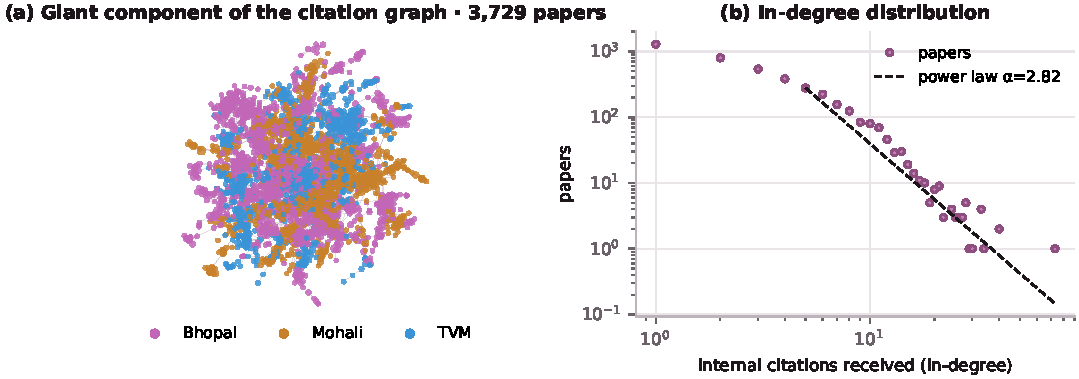
\includegraphics[width=\linewidth]{figures/fig_citation.pdf}
\caption{(a) Giant weakly connected component of the internal citation graph (nodes = papers, size $\propto$ PageRank, colour = institute). (b) In-degree distribution on log--log axes with the best power-law fit for reference.}
\label{fig:cit}
\end{figure}

The directed graph has \CNodes{} papers and \CEdges{} internal citation edges (``paper A cites paper B'', both authored by our faculty). The raw \texttt{citation\_network.csv} also carries \COutIndia{} outgoing and \CInIndia{} incoming edges to and from other Indian institutes. About half the papers (\CGiant) sit in one weakly connected component, and the median citation lag is \CLag{} years. \CSelf{} of internal edges join two papers of the \emph{same} institute: the three IISERs barely build on each other's work.

The in-degree distribution is heavy-tailed. A power law fits above $x_{\min}=\CXmin$ with $\alpha=\CAlpha$, but a log-normal fits significantly better (likelihood ratio $R=\CRLN$, $p<0.001$), the usual signature of cumulative advantage tempered by ageing rather than pure preferential attachment. PageRank (Table~\ref{tab:pr}) surfaces papers that are cited by \emph{well-cited} internal papers: Bhopal's noncentrosymmetric-superconductor line and Mohali's atmospheric-chemistry papers outrank far more cited papers, because they seed long internal citation chains. The Planck 2018 entry ranks highly only because the papers in that series cite one another, which is why the dashboard offers a ranking without large collaborations.

\begin{table}[!htb]
\centering\footnotesize
\caption{PageRank top 10 on the internal citation graph ($\alpha=0.85$); \emph{in} = citations from other corpus papers.}
\label{tab:pr}
\begin{tabularx}{\linewidth}{@{}r X r l r r@{}}
\toprule
\# & Title & Year & Inst. & In & All cites \\
\midrule
1 & Superconducting properties of the noncentrosymmetric supercondu… & 2016 & Bhopal & 20 & 57 \\
2 & Time-reversal symmetry breaking in the noncentrosymmetric super… & 2017 & Bhopal & 33 & 83 \\
3 & Overview of VOC emissions and chemistry from PTR-TOF-MS measure… & 2016 & Mohali & 14 & 116 \\
4 & Contribution of post-harvest agricultural paddy residue fires i… & 2016 & Mohali & 27 & 104 \\
5 & Strong interlayer coupling mediated giant two-photon absorption… & 2016 & Bhopal & 28 & 71 \\
6 & Planck 2018 results & 2020 & TVM & 73 & 14,257 \\
7 & Trace level detection of nitroanilines using a solution process… & 2016 & Bhopal & 11 & 102 \\
8 & Crystal-to-Crystal Synthesis of Triazole-Linked Pseudo-proteins… & 2016 & TVM & 44 & 80 \\
9 & Dynamical Phase Transition in Neutron Stars & 2018 & Bhopal & 15 & 19 \\
10 & Effect of magnetic field on the burning of a neutron star & 2018 & Bhopal & 6 & 7 \\
\bottomrule

\end{tabularx}
\end{table}

\section{Co-authorship network}
\begin{figure}[!htb]
\centering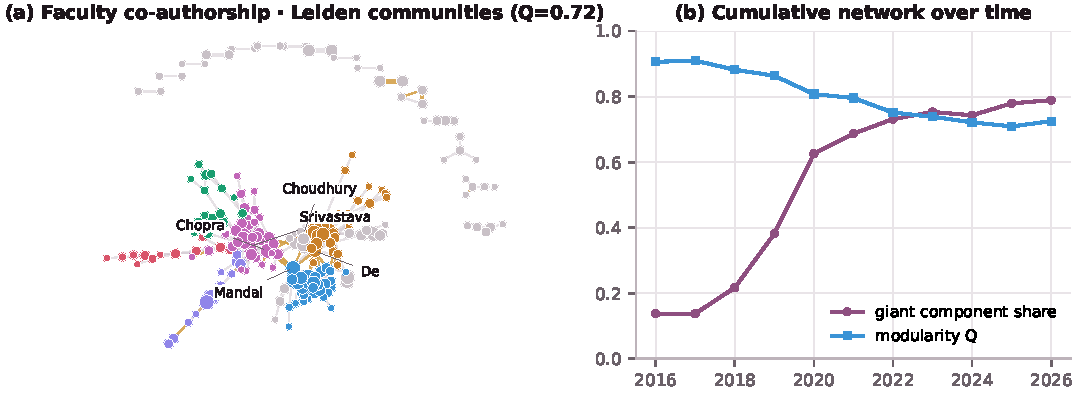
\includegraphics[width=\linewidth]{figures/fig_coauthor.pdf}
\caption{(a) Faculty co-authorship network (papers with $\le$\HyperCap{} authors; node size = joint papers; gold edges cross institutes; the six largest Leiden communities coloured, the five strongest brokers named). (b) Cumulative network by year.}
\label{fig:co}
\end{figure}

Nodes are our \ANodes{} matched faculty, joined when they co-authored a paper (weight = joint papers). Only \AConn{} faculty have a co-author among the other faculty; the remaining \AIso{} collaborate only with students, postdocs or outsiders. The \AEdges{} ties form a sparse (mean degree \AMeanDeg) but strongly clustered network. Its clustering of \AC{} is \ACratio{} times the configuration-model value (\ACnull) at a similar path length (\AL{} vs \ALnull), giving small-world $\sigma=\ASigma$ (90\% of 50 null graphs give \ASigmaLo--\ASigmaHi, all well above 1). Leiden finds \ALeiden{} communities with modularity $Q=\AQ$ (Louvain \ALouvQ). They agree only partly with departments (NMI \ANMI, ARI \AARI): the large communities are \emph{interdisciplinary within one institute}, for example Bhopal chemistry with biology, and TVM chemistry with physics.

Brokers with the highest betweenness are \ABtwA, \ABtwB{} and \ABtwC{} (Table~\ref{tab:central}). From \AYearStart{} to \AYearEnd{} the giant component grew from \AGiantStart{} to \AGiantEnd{} of connected faculty while modularity fell from \AModStart{} to \AModEnd{} (Fig.~\ref{fig:co}b): the network is knitting together without losing its group structure. As a first model we predicted which faculty pairs would \emph{start} collaborating after \LPSplit{} from the network up to \LPSplit. Preferential attachment (AUC \LPPA) and same-department membership (\LPDept) beat common-neighbour scores such as Adamic--Adar (\LPAA): new ties go to already well-connected people in the same department more than to friends of friends.

\begin{table}[!htb]
\centering\footnotesize
\caption{Most collaborative (degree) and most bridging (weighted betweenness) faculty.}
\label{tab:central}
\begin{tabular}{@{}r l r l r@{}}
\toprule
\# & Degree & $k$ & Betweenness & $b$ \\
\midrule
1 & Deepak Chopra (Bhopal) & 13 & Deepak Chopra (Bhopal) & 0.099 \\
2 & Santanu Kumar Pal (Mohali) & 13 & Sukhendu Mandal (TVM) & 0.076 \\
3 & Sukhendu Mandal (TVM) & 13 & Aasheesh Srivastava (Bhopal) & 0.048 \\
4 & Arijit Kumar De (Mohali) & 10 & Arijit Kumar De (Mohali) & 0.044 \\
5 & Joy Mitra (TVM) & 10 & Angshuman Roy Choudhury (Mohali) & 0.028 \\
6 & Ram Kumar Mishra (Bhopal) & 9 & Kausik Chattopadhyay (Mohali) & 0.022 \\
7 & Aasheesh Srivastava (Bhopal) & 9 & J. Sankar (Bhopal) & 0.020 \\
8 & M M Shaijumon (TVM) & 9 & Sanjay Singh (Mohali) & 0.020 \\
\bottomrule

\end{tabular}
\end{table}

\section{Indian connectivity}
\begin{figure}[!htb]
\centering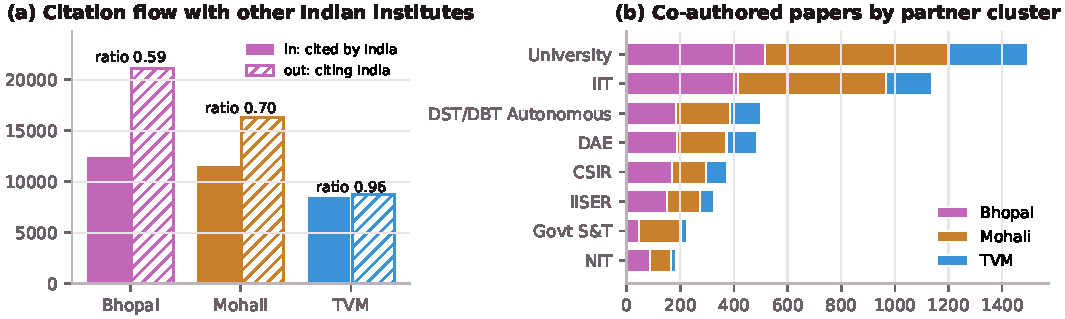
\includegraphics[width=\linewidth]{figures/fig_connect.pdf}
\caption{(a) Citations exchanged with other Indian institutes: in = an Indian-authored paper cites ours, out = our paper cites one; the in/out ratio is printed above each pair. (b) Co-authored papers by partner cluster.}
\label{fig:conn}
\end{figure}

Our faculty co-author with \Partners{} other Indian institutes, and \Linked{} Indian institutes are linked to them by co-authorship or citation. Bhopal received \InB{} citations from other Indian institutes and gave \OutB{} (ratio \RatioB); Mohali \InM{} vs \OutM{} (\RatioM); TVM \InT{} vs \OutT{} (\RatioT). The ratio is partly a time effect: references are complete at publication, while incoming citations keep arriving. The most frequent Indian citer of Bhopal and Mohali is the Academy of Scientific and Innovative Research (CSIR's PhD-granting academy), and of TVM the Homi Bhabha National Institute (DAE). The strongest co-authorship partners are IIT Kanpur (Bhopal), TIFR (Mohali) and IISc (TVM). By cluster, universities and IITs dominate shared papers, followed by DST/DBT autonomous institutes, DAE and CSIR; these \emph{cross-cluster} links (IISER$\leftrightarrow$IIT, IISER$\leftrightarrow$CSIR/DAE) far outnumber IISER$\leftrightarrow$IISER papers. Topic overlap (Jaccard on the top-50 OpenAlex topics) with each partner is in \texttt{indian\_connections.csv} and on the dashboard.

\section{Why these findings matter}
\begin{itemize}
\item \textbf{Raw counts mislead in exactly the places where rankings use them.} One Planck release decides which IISER looks ``most cited''. Any comparison of these institutes (NIRF-style or internal) should use field-weighted impact and report large-collaboration papers separately, as this dashboard does.
\item \textbf{The IISER system is three parallel systems.} With \CSelf{} of mutual citations inside one institute and only \ACross{} cross-IISER faculty ties, the three institutes work largely in isolation from each other. Their subfield portfolios overlap substantially (weighted Jaccard \SimLo--\SimHi; dashboard: Research Areas), so the missing links are an opportunity rather than a mismatch. Joint centres or shared PhD supervision could target the faculty pairs the link-prediction model ranks highest.
\item \textbf{Collaboration is organised around people, not departments.} Communities cut across Chemistry, Biology and Physics inside each campus, and a few brokers (Table~\ref{tab:central}) hold large parts of the network together. That is a strength for interdisciplinary work and a fragility if those people leave.
\item \textbf{The IISERs are absorbers of Indian science.} They cite universities, IITs and DAE/CSIR labs more than these cite them back. As the institutes mature (TVM is already near balance), the ratio is a simple indicator of whether they become sources of Indian knowledge rather than only consumers.
\end{itemize}

\section{What the second round will add}
\begin{itemize}
\item \textbf{Better community models.} A degree-corrected (nested) stochastic block model will test whether the institute/department structure is real or a modularity artefact, and core--periphery detection will find a collaborative core.
\item \textbf{Temporal and disruption measures.} We will compute the CD disruption index and identify ``sleeping beauty'' papers on the citation graph, and fit a citation model with preferential attachment, ageing and fitness to explain the log-normal tail.
\item \textbf{Representation learning for link prediction.} Node2vec embeddings plus topic similarity, evaluated on the same temporal split, to recommend cross-IISER collaborations where topics overlap but no ties exist (the three portfolios share a large part of their subfield mix).
\item \textbf{A multilayer view.} Combine the citation, co-authorship and topic-similarity layers, and extract the disparity-filter backbone of the Indian partner network.
\end{itemize}

\end{document}
